\chapter{Mengenal Kecerdasan Buatan dan Scikit-Learn}
Buku umum yang digunakan adalah \cite{russell2016artificial} dan  
untuk sebelum UTS menggunakan buku \textit{Python Artificial Intelligence Projects for Beginners}\cite{eckroth2018python}.
Dengan praktek menggunakan python 3 dan editor anaconda dan library python scikit-learn.
Tujuan pembelajaran pada pertemuan pertama antara lain:
\begin{enumerate}
\item
Mengerti definisi kecerdasan buatan, sejarah kecerdasan buatan, perkembangan dan penggunaan di perusahaan
\item
Memahami cara instalasi dan pemakaian sci-kit learn
\item
Memahami cara penggunaan variabel explorer di spyder
\end{enumerate}
Tugas dengan cara dikumpulkan dengan pull request ke github dengan menggunakan latex pada repo yang dibuat oleh asisten riset.

\section{Teori}
Praktek teori penunjang yang dikerjakan :
\begin{enumerate}
\item
Buat Resume Definisi, Sejarah dan perkembangan Kecerdasan Buatan, dengan bahasa yang mudah dipahami dan dimengerti. Buatan sendiri bebas plagiat[hari ke 1](10)
\item
Buat Resume mengenai definisi supervised learning, klasifikasi, regresi dan unsupervised learning. Data set, training set dan testing set.[hari ke 1](10)
\end{enumerate}

\section{Instalasi}
Membuka https://scikit-learn.org/stable/tutorial/basic/tutorial.html. Dengan menggunakan bahasa yang mudah dimengerti dan bebas plagiat. 
Dan wajib skrinsut dari komputer sendiri.
\begin{enumerate}
\item
Instalasi library scikit dari anaconda, mencoba kompilasi dan uji coba ambil contoh kode dan lihat variabel explorer[hari ke 1](10)
\item
Mencoba Loading an example dataset, menjelaskan maksud dari tulisan tersebut dan mengartikan per baris[hari ke 1](10)
\item
Mencoba Learning and predicting, menjelaskan maksud dari tulisan tersebut dan mengartikan per baris[hari ke 2](10)
\item
mencoba Model persistence, menjelaskan maksud dari tulisan tersebut dan mengartikan per baris[hari ke 2](10)
\item 
Mencoba Conventions, menjelaskan maksud dari tulisan tersebut dan mengartikan per baris[hari ke 2](10)
\end{enumerate}


\section{Penanganan Error}
Dari percobaan yang dilakukan di atas, apabila mendapatkan error maka:

\begin{enumerate}
	\item
	skrinsut error[hari ke 2](10)
	\item
Tuliskan kode eror dan jenis errornya [hari ke 2](10)
	\item
Solusi pemecahan masalah error tersebut[hari ke 2](10)

\end{enumerate}

\section{Teori/Fadila/1164072}
Teori mencakup resume dari beberapa pembahasan. yaitu :
\begin{enumerate}
\item Tentang Kecerdasan Buatan
\begin{itemize}
\item Definisi Kecerdasan Buatan.
\par Kecerdasan Buatan biasa disebut dengan istilah AI ( Artificial Intelligence ) . AI sendiri merupakan suatu cabang dalam bidang sains komputer sains dimana mengkaji tentang bagaimana cara untuk melengkapi sebuah komputer dengan kemampuan atau kepintaran layaknya atau mirip dengan yang dimiliki manusia. Sebagai contoh, sebagaimana komputer dapat berkomunikasi dengan pengguna baik menggunakan kata, suara maupun lain sebagainya . Dengan kemampuan ini, diharapkan komputer mampu mengambil keputusan sendiri untuk berbagai kasus yang ditemuinya kemudian itulah yang disebut dengan kecerdasan buatan.
\par  Kecerdasan buatan makin canggih dengan kemampuan komputer dalam memperbarui pengetahuannya dengan banyaknya testing dan perkembangan target analisa. Untuk kecerdasan buatan ada banyak contoh dan jenisnya. Salah satu contoh yang paling terkenal dari Artificial Intelligence ialah Google Assistant. Google Assistant digunakan untuk kemudahan user dalam menemukan berbagai hal maupun penyettingan langsung terhadap smartphone yang digunakan dan masih banyak lagi.
\item Sejarah Kecerdasan Buatan
\par Artificial intelligence merupakan inovasi baru di bidang ilmu pengetahuan. Mulai terbentuk sejak adanya komputer modern dan kira-kira terjadi sekitaran tahun 1940 dan 1950. Ilmu pengetahuan komputer ini khusus ditujukan dalam perancangan otomatisasi tingkah laku cerdas dalam sistem kecerdasan komputer. 
\par Pada awalnya, kecerdasan buatan hanya ada di universitas-universitas dan laboratorium penelitian, serta hanya sedikit produk yang dihasilkan dan dikembangkan. Menjelang akhir 1970-an dan 1980-an, mulai dikembangkan secara penuh dan hasilnya berangsur-angsur dipublikasikan di khalayak umum. 
\par

\begin{figure}[ht]
\centering
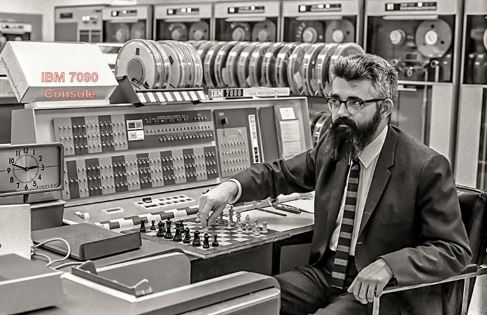
\includegraphics[scale=0.5]{figures/contoh.jpg}
\caption{capturing}
\label{contoh}
\end{figure}

\par Jika kita berbicara tentang AI atau Artificial Intelligence maka kita tidak bisa melupakan seorang sosok yang sangat terkenal pada bidang tersebut yaitu bapak John McCarthy. 
McCarthy mendapatkan gelar sarjana matematika dari California Institute of Technology (Caltech) pada September 1948. Dari masa kuliahnya itulah ia mulai mengembangkan ketertarikannya pada mesin yang dapat menirukan cara berpikir manusia. McCarthy kemudian melanjutkan pendidikan ke program doktoral di Princeton University.

\par McCarthy kemudian mendirikan dua lembaga penelitian kecerdasan buatan. Kedua lembaga AI itu adalah Stanford Artificial Intelligence Laboratory dan MIT Artificial Inteligence Laboratory. Di lembaga-lembaga inilah bermunculan inovasi pengembangan AI yang meliputi bidang human skill, vision, listening, reasoning dan movement of limbs. Bahkan Salah satu lembaga yang didirikan itu, Stanford Artificial Intelligence pernah mendapat bantuan dana dari Pentagon untuk membuat teknologi-teknologi luar angkasa.

\item Perkembangan Kecerdasan Buatan
\par Teknologi Artificial Intelligence semakin ramai dibahas dalam berbagai diskusi teknologi di seluruh dunia.Menurut kebanyakan orang, pekerjaan seperti kasir, operator telepon, pengendara truk, dan lainnya sangat berpeluang besar untuk tergantikan oleh Artificial Intelligence. Mengapa terjadi hal demikian? dikarenakan memang bahwa AI lebih ungul dalam hal kinerja, fitur dan lain sebagainya. Namun, dalam beberapa aspek memang pekerja manusia masih unggul dibandingkan AI itu sendiri.
\par Para generasi muda yang ada di dunia terutama di daerah Asia terlihat sudah memahami fungsi dan efek dari AI dalam kehidupan kita sehari-hari. Berdasarkan survei yang dilakukan oleh Microsoft, terdapat 39 persen responden yang mempertimbangkan untuk menggunakan mobil tanpa pengemudi dan 36 persen lainnya setuju bahwa robot masa depan dengan software untuk beroperasi mampu meningkatkan produktivitas. Dari survey tersebut kita sebagai pengguna AI harus lebih bijaksana dalam pengembangan dan penggunaan dari AI sehingga tanpa memberikan efek samping terhadap etos kerja dan keseharian kita sebagai pengguna dalam kehidupan sehari-hari.
\end{itemize}
\item Tentang Pengertian Terhadap Ilmu Yang Lain
\begin{itemize}
\item Supervised Learning adalah pendekatan dimana sudah terdapat data yang dilatih selain itu juga terdapat variable yang ditargetkan sehingga tujuan dari pendekatan ini yaitu mengkelompokan suatu data ke data yang sudah ada.
\par
\item Klasifikasi adalah pembagian sesuatu menurut kelas-kelas ( class ). Menurut Ilmu Pengetahuan, Klasifikasi merupakan proses pengelompokkan benda berdasarkan ciri-ciri persamaan dan juga perbedaan.
\par
\item Regresi adalah metode analisis statistik yang digunakan untuk melihat pengaruh antara dua ataupun lebih variabel.
\par
\item Unsupervised Learning berbeda dengan Supervised Leraning. Perbedaannya ialah unsupervised learning tidak memiliki data latih, sehingga dari data yang ada kita mengelompokan data tersebut menjadi 2  ataupun 3 bagian dan seterusnya.
\par
\item Dataset adalah objek yang merepresentasikan data dan juga relasi yang ada di memory. Strukturnya mirip dengan data di database, namun bedanya dataset berisi koleksi dari data table dan data relation. 
\par
\item Training Set adalah set digunakan oleh algoritma klassifikasi . Dapat dicontohkan dengan :  decision tree, bayesian, neural network dll. Semuanya dapat digunakan untuk membentuk sebuah model classifier. 
\par
\item Testing Set adalah set yang digunakan untuk mengukur sejauh mana classifier berhasil melakukan klasifikasi dengan benar. 
\par
\end{itemize}
\end{enumerate} 


\section{Instalasi/Fadila/1164072)}
Untuk Instalasinya mencakup i beberapa pembahasan dan tutorial. yaitu :
\begin{enumerate}
\item Instalasi Scikit-Learn Dari Anaconda 
\begin{itemize}
\item Instalasi Anaconda
\begin{enumerate}
\item Pertama-tama silahkan pastikan bahwa anda telah melakukan instalasi software Anaconda.
\item Apabila belum, silahkan buka web browser anda untuk melakukan pengunduhan software Anaconda
\item Setelah terunduh, silahkan klik kanan lalu run administrator pada software Anaconda
\item Silahkan lakukan penginstalan dengan menekan tombol install pada tampilan instalasi
\item Kemudian tekan tombol next maka akan sampai pada tampilan diatas

\par

\begin{figure}[ht]
\centering
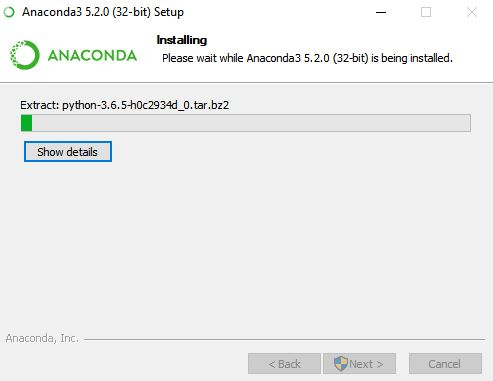
\includegraphics[scale=0.5]{figures/ana1.jpg}
\caption{install anaconda 1}
\label{contoh}
\end{figure}

\par
\item Selanjutnya apabila instalan tersebut telah selesai maka silahkan menekan tombol next
\item Tampilan selanjutnya akan seperti ini

\par

\begin{figure}[ht]
\centering
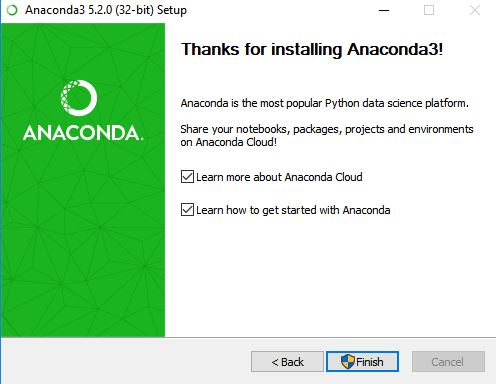
\includegraphics[scale=0.5]{figures/ana2.jpg}
\caption{install anaconda 2}
\label{contoh}
\end{figure}

\par

\item Apabila tampilannya telah sesuai dengan contoh gambar maka instalasi telah selesai
\end{enumerate}
\end{itemize}

\begin{itemize}
\item Instalasi Library Scikit Learn
\begin{enumerate}
\item Silahkan membuka web browser untuk melakukan pengunduhan untuk library scikit dari anaconda.
\item Silahkan mengunjungi halaman ini untuk melakukan pengunduhan library scikit dari anaconda.
\par https://anaconda.org/anaconda/scikit-learn.
\item Setelah terdownload silahkan melakukan instalasi lanjutan menggunakan Command Prompt
\item Silahkan masukkan perintah berikut untuk melakukan pengecekan bahwa anaconda anda telah terpasang dengan baik.
\par conda --version
\par python --version
\item Tampilannya akan nampak seperti berikut :
\par

\begin{figure}[ht]
\centering
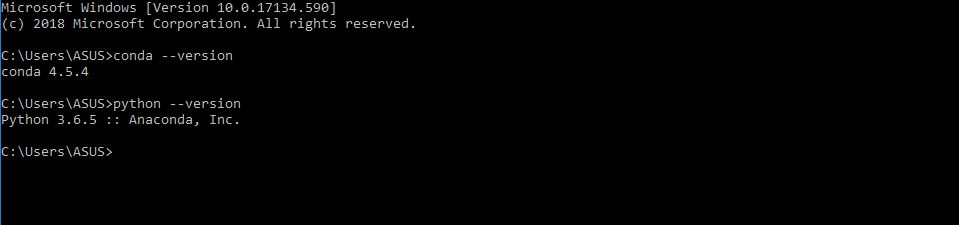
\includegraphics[scale=0.3]{figures/scikit1.jpg}
\caption{Pengecekan Anaconda}
\label{contoh}
\end{figure}

\par
\item Selanjutnya silahkan masukkan perintah berikut untuk melakukan instalasi pip sckit-learn
\par perintahnya : pip install -U scikit-learn
\item Tampilannya akan nampak seperti berikut :
\par

\begin{figure}[ht]
\centering
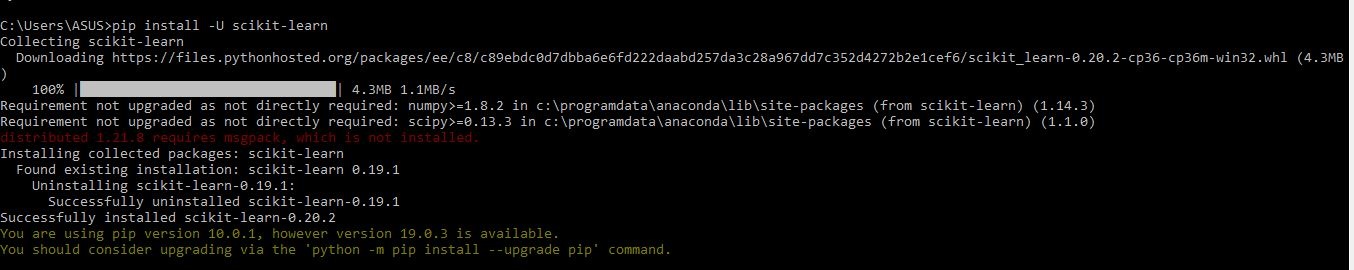
\includegraphics[scale=0.2]{figures/scikit3.jpg}
\caption{instalasi pip scikit-learn}
\label{contoh}
\end{figure}

\par
\item Selanjutnya silahkan masukkan perintah berikut untuk melakukan instalasi conda sckit-learn
\par perintahnya : conda install scikit-learn
\item Tampilannya akan nampak seperti berikut :
\par

\begin{figure}[ht]
\centering
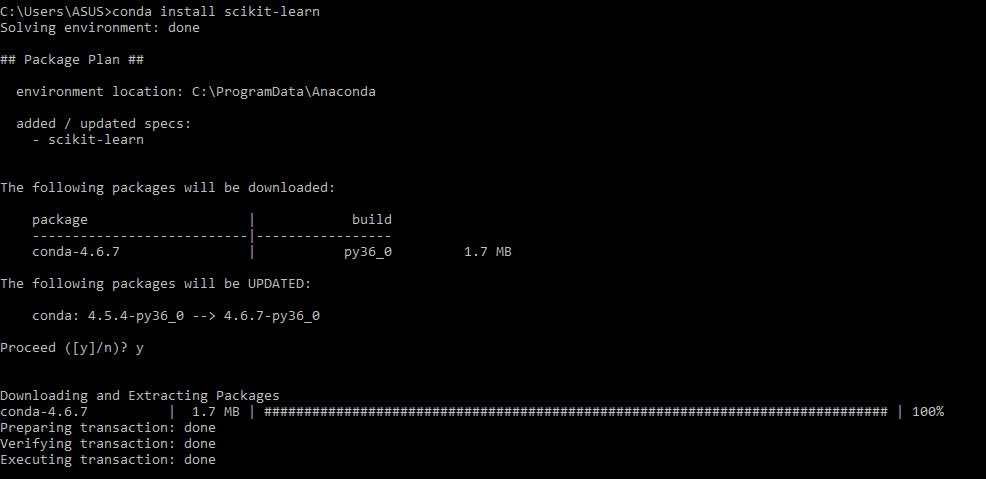
\includegraphics[scale=0.3]{figures/scikit4.jpg}
\caption{instalasi conda scikit-learn}
\label{contoh}
\end{figure}

\par
\par
\par
\item Apabila telah dipraktekan seperti langkah-langkah dan menghasilkan tampilan seperti contoh diatas, maka instalasi scikit-learn dari anaconda berhasil dilakukan
\par
\item Kemudian untuk pengujian yang lain yaitu pengujian untuk mengecek codingan anaconda
\par
\item Contoh uji coba codingannya dapat dilihat pada gambar berikut
\par
\begin{figure}[ht]
\centering
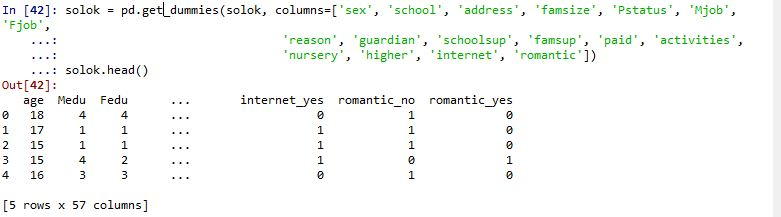
\includegraphics[scale=0.5]{figures/3.jpg}
\caption{uji coba codingan}
\label{contoh}
\end{figure}
\par
\item Berdasarkan pengujian tersebut maka dapat dipastikan bahwa anaconda telah ter-include ke dalam python dan dieksekusi dengan script python
\item Setelah pengeksekusiannya berdasarkan scripts python, terdapatlah keluaran yang sesuai 
\item Keluaran tersebut yang menandakan bahwa anacondanya berfungsi dengan baik.
\end{enumerate}
\end{itemize}


\par
\item Loading An Example Dataset
\begin{itemize}
\item Penerapan Loading An Example Dataset Pada Python Di CMD
\begin{enumerate}
\item Pertama-tama silahkan buka command prompt di laptop anda
\item Selanjutnya masuk ke python 
\item Setelah masuk kedalam python, silahkan masukkan perintah seperti pada gambar berikut :

\begin{figure}[ht]
\centering
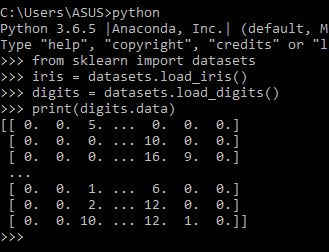
\includegraphics[scale=0.6]{figures/4.jpg}
\caption{pengujian loading an example dataset}
\label{contoh}
\end{figure}

\par 
\item Secara keseluruhan, hasilnya pada command prompt akan nampak seperti gambar tersebut
\item Apabila tampilanya telah nampak seperti gambar diatas, maka pengujiannya telah selesai dan berhasil.
\end{enumerate}

\par
\item Penjelasan Perintah Yang Di Uji
\begin{enumerate}
\item Perhatikan perintah yang telah dieksekusi ini :

\par
\begin{figure}[ht]
\centering
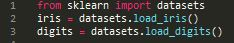
\includegraphics[scale=0.9]{figures/ok4.jpg}
\caption{pengujian loading an example dataset}
\label{contoh}
\end{figure}
\par

\item Penjelasan untuk baris pertama ialah : 
\par Perintahnya yaitu memasukkan dan memanggil dataset dari sklearn
\par
\par
\item Penjelasan untuk baris kedua ialah :
\par Terdapat variabel baru yaitu iris. Dimana variabel iris memanggil datasets dan di dalamnya akan ngeload ( menampilkan ) load iris.
\par
\item Penjelasan untuk baris ketiga ialah :
\par Kemudian ada juga variabel baru lainnya yaitu digits yang akan memanggil dataset dan di dalamnya akan ngeload ( menampilkan ) load digits
\par
\item Selanjutnya untuk perintah Print( digits.data ) ditujukan untuk me-
\par nampilkan output dari pengeksekusian variabel digits dan akan berupa data.
\par
\item Hasilnya printnya sebagai berikut :
\par

\begin{figure}[ht]
\centering
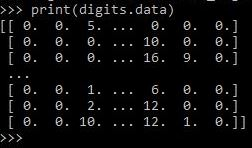
\includegraphics[scale=0.7]{figures/okk4.jpg}
\caption{hasil print uji cobat}
\label{contoh}
\end{figure}

\par
\item Untuk penjelasan uji cobanya sudah selesai.
\par
\end{enumerate}
\end{itemize}
\end{enumerate}